\documentclass[class=article, crop=false]{standalone}
\usepackage{my_preamble}
\begin{document}
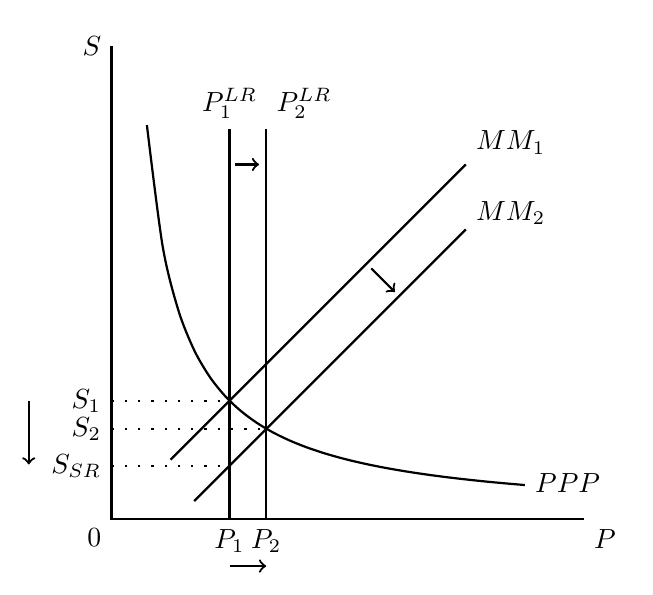
\begin{tikzpicture}[thick,font=\sffamily,scale=1.5]
	%axis and labels
	 \draw (0,4) node[left]{$S$} -- (0,0) node[below left] {$0$} 
	  -- (4,0) node[below right]{$P$};
	  
	%graphs
	\draw plot[domain=0.5:3,smooth] (\x,\x); %Mm
	\draw plot[domain=0.3:3.5,smooth] (\x,1/\x); %PPP
	\draw[] (1,0) -- (1,3.3); %LR prices

	%labels
	\node[right] at (3.5,0.3) {$PPP$}; %PPP label
	\node[above] at (1,3.3) {$P^{LR}_1$}; %MM label  
	\node[above right] at (3,3) {$MM_{1}$}; %LR prices label  
	
	%dotted lines
	 \draw[loosely dotted] (0,1) node[left]{$S_1$} -| node[pos=0.25,below=3mm] {}
  (1,0) node[below]{$P_1$}; %S1 and P1

%shift-------------------------------------------------------------
	%graphs
	\draw plot[domain=0.7:3,smooth] (\x,\x-0.55); %MM2
	\draw[] (1.31,0) -- (1.31,3.3); %LR prices 2

	%labels
	\node[above right] at (1.31,3.3) {$P^{LR}_2$}; %MM2 label   
	\node[above right] at (3,2.4) {$MM_{2}$}; %LR prices 2 label
	
	%dotted lines
	 \draw[loosely dotted] (0,0.76) node[left]{$S_2$} -| node[pos=0.25,below=3mm] {}
  (1.31,0) node[below]{$P_2$}; %S2 and P2
  \draw[loosely dotted] (0,0.45) node[left]{$S_{SR}$} -| node[pos=0.25,below=3mm] {}
  (1,0) node[below]{}; %x3 and horizontal lines
    
	%arrows
	\draw [->] (1,-0.4) -- (1.31,-0.4); %x arrow
	\draw [->] (-0.7,1) -- (-0.7,0.46); %y arrow
	\draw [->] (1.05,3) -- (1.25,3); %LR prices arrow
	\draw [->] (2.2,2.12) -- (2.4,1.92); %MM arrow

%---------------------------------------------------------------
%ALTERNATIVE GRAPHS	
	%\draw [thick, name path = F1] (0.2,3.5) to [out=270,in=180] (3.5,0.2); %PPP
	%\draw[] (1.15,0) -- (1.15,3); %LR prices
	
\end{tikzpicture}
\end{document}